\documentclass[12pt]{article}

\usepackage[margin=3cm]{geometry}
\usepackage{graphicx}
\usepackage{pdfpages}
\usepackage{minted}

\author{Pablo Vargas Bermúdez}

\begin{document}
\pagestyle{empty}

\includepdf[pages=-]{Portada}

\section*{Descripción}
Usando los objetos JMenuBar, JMenu y JMenuItem Cree un esqueleto de
menu similar al siguiente:

\begin{center}
  \includegraphics[width=.5\textwidth]{figures/show.png}
\end{center}

En el libro: Pensando en Java de Bruce Eckel podrás encontrar una
descripción del armado y funcionamiento de menus.

Envía un archivo PDF que contenga una hoja de presentación, la
descripción de la tarea, el código fuente de la solución y las
capturas de pantalla necesarias donde muestres el correcto
funcionamiento del programa

\section*{Código}
\inputminted{Java}{Gui.java}
\inputminted{Java}{Prueba.java}

\section*{Ejecución}
\begin{figure}[ht]
  \centering
  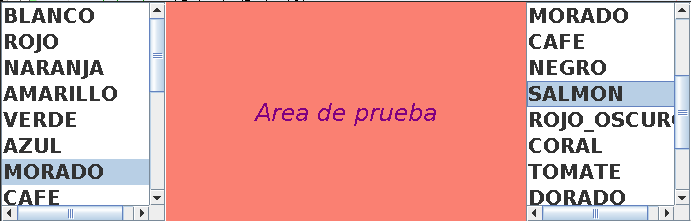
\includegraphics[width=\textwidth]{figures/run1.png}
  \caption{Resultado del Menu}
\end{figure}

\end{document}
